%----------------------------------------------------------------------------------------
%	PACKAGES AND DOCUMENT CONFIGURATIONS
%----------------------------------------------------------------------------------------
\documentclass[11pt]{article}
\usepackage{amsmath} % Required for some math elements
\usepackage{hyperref} 
\usepackage{xcolor}
\usepackage{lipsum} 
\usepackage{cite}
\usepackage{graphicx} % Required for the inclusion of images
\usepackage{algorithmic}
\usepackage{array}
\usepackage{bookmark}
\usepackage{listings}
\usepackage{amssymb}
\usepackage{enumitem}   
\usepackage[margin=16mm]{geometry}
\usepackage[caption=false, font=footnotesize]{subfig}
\usepackage{multirow}
\usepackage[active,tightpage]{preview}

\renewcommand{\PreviewBorder}{1in}
\newcommand{\Newpage}{\end{preview}\begin{preview}}

\newlist{steps}{enumerate}{1}
\setlist[steps, 1]{label = Step \arabic*:}

\hypersetup{ %color attributes of citation, link, etc.
    colorlinks=true,
    linkcolor=blue,
    filecolor=gray,      
    urlcolor=blue,
    citecolor=blue,
}

\newcommand{\matlab}{\textsc{Matlab}} %very important and totally necessary addition

\newcommand\Item[1][]{%
  \ifx\relax#1\relax  \item \else \item[#1] \fi
  \abovedisplayskip=0pt\abovedisplayshortskip=0pt~\vspace*{-\baselineskip}}
%----------------------------------------------------------------------------------------
%	DOCUMENT INFORMATION
%----------------------------------------------------------------------------------------
 
\title{ECEN321: Analogue Electronics \\ Assignment 2 \\ Thermal Analysis and Voltage Regulation - Submission}
\author{Daniel Eisen : 300447549}
\date{\today}

\begin{document}
\begin{preview}

\maketitle
%----------------------------------------------------------------------------------------
%	DOCUMENT CONTENT
%----------------------------------------------------------------------------------------
\section*{Question 1:}
\begin{enumerate}[label=\alph*)]
  % Explain the purpose of heat sinks. Also, why do we include an insulating washer between the transistor and the heat sink?
          \item  Heat Sinks are uses to lower the junction temperature by transferring heat from the junction to ambient. This provides mitigation of the degradation of characteristics and prevent failure due to thermal cycling. The insulating washer provides electrical insulation as well as thermal conductivity.
% What is the difference between LM7806 andLM7912?
          \item Both are three terminal, fixed voltage regulators. \\
          The LM7806 provides an output of +6V for a minimum $V_i$ of +8.3\\
          The LM7912 provides an output of -12V for a minimum $V_i$ of -14.6\\
          i.e differences being 78XX is positive out for positive in, and 79XX is negative out for negative in.
% What are the basic types of switching regulators and how do they differ? What are the basic difference between switching and linear regulators and where do we use them?    
          \item The three types of switching regulators are step-up (boost), step-down (buck), and inverting:
          \\ Step-Up: V-out is always greater than V-in, Step-down: V-out always lower that V-in, Inverting inverted the polarity of the input voltage but can be at any relative level. \\ Switching have max efficiencies of $\ge90\%$ where linear can only much less, especially when the output varies far from the input. Linear are cheaper, so used in lower current application, where efficiency/energy loss isn't that much an issue. Usually when the output is closer to the input. Switching is particularly good for high current applications due to high efficiencies but are harder to control the output noise.
          \item \begin{itemize}
            \item Required input and out voltages
            \item Total current requirements of the supplied circuit
            \item Efficiency
            \item How much filtering is needed
            \item The noise allowances when using a switching supply 
          \end{itemize}
\end{enumerate}

\section*{Question 2:}
\begin{enumerate}[label=\alph*)]
          \item $115-(90-25)*0.657=72.295W$
          \Item \\ 
          \textbf{COMPONENTS:}

          Chose STP16NF06 a 60V - 16A, Power MOSFET\\
          \begin{tabular}{llll}
            \textbf{Symbol} & \textbf{Parameter}                                  & \textbf{Value}              & \textbf{Unit}              \\
            $T_{stg}$           & Storage temperature                             & \multirow{2}{*}{-55 to 175} & \multirow{2}{*}{$^\circ$C} \\
            $T_{j}$             & Max. operating junction temperature             &                             &                            \\
            $R_{th-case}$        & Thermal resistance junction-case max           & 3.33                        & $^\circ$C/W                \\
            $R_{th-amb}$         & Thermal resistance junction-ambient max        & 62.5                        & $^\circ$C/W                \\
            $T_{J}$              & Maximum lead temperature for soldering purpose & 300                         & $^\circ$C                     
          \end{tabular} 

          Chose F series heatsink, FA-T220-64E (2.5" Height, 46g, 22,814mm$^2$) \\

          \textbf{ANALYSIS:}

          $P_d = 13W, \; T_{a-max} = 50^{\circ}C, \; R_{\Theta jc} = 3.33^{\circ}C/W, \; R_{\Theta ja} = 62.5^{\circ}C/W$ 

          \textbf{Without heatsink:}
          \begin{align*}
          T &= R_{\Theta ja} {\cdot} P_d + T_{a-max} \\
          &= (62.5 \times 13)+50 \\
          T &= 862.5^{\circ}C
          \end{align*}
          So definatly requires further thermal management. \\

          \textbf{With Heatsink (+thermal grease):}

          \begin{center}
            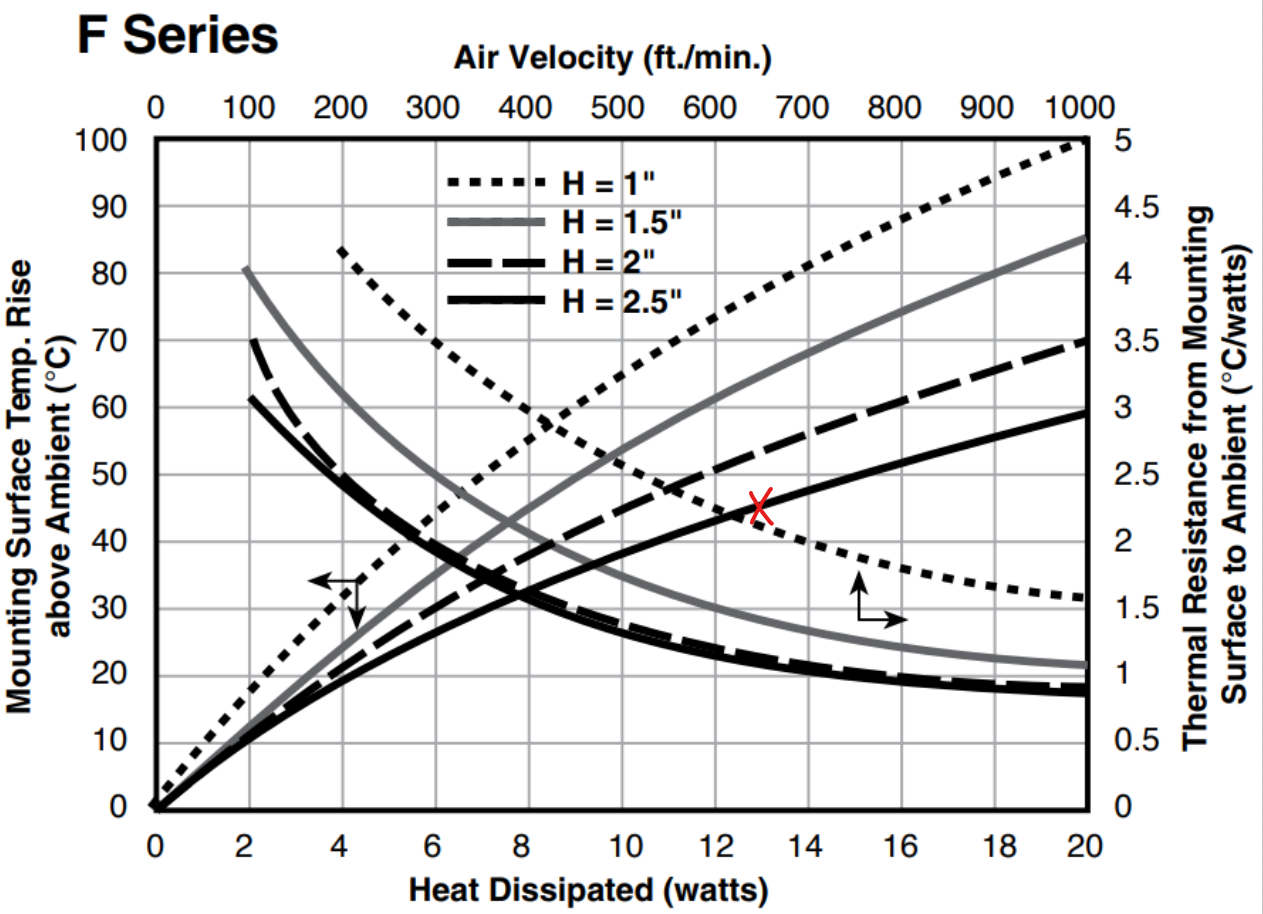
\includegraphics[width=0.3\textwidth]{F_series_heatsink_natural.png}
          \end{center}

          So for our power dissipation of 13W, the temperature rise corresponds to 45$^\circ$C (i.e for the curve H=2.5").

          For an included safety factor of 20\%:
          \begin{align*}
            R_{\Theta sa} &= (T_{r} / P_{d}) \times 1.2 \\
            &= (45/13) \times 1.2\\
            R_{\Theta sa} &=4.153846^{\circ}C/W
          \end{align*}
          Then using a thermal grease with an assumed $R_{\Theta cs} = 0.2^{\circ}C/W$
          \begin{align*}
            T_{s} &= R_{\Theta sa} \times P_{d} + T_{a}\\
                  &= 4.15*13+50=103.95 \\
            T_{c} &= R_{\Theta cs} \times P_{d} + T_{s} \\
                  &= 0.2*13+103.95=106.55 \\
            T_{j} &= R_{\Theta jc} \times P_{d} + T_{c} \\
                  &= 3.33*13+106.55 \\ 
            T     &= 149.84^{\circ}C
          \end{align*}
          So with a natural convection heatsink, the temperature is reduced to below the max operating temperature, but only just.

          \textbf{With Forced Convection:}

          \begin{center}
            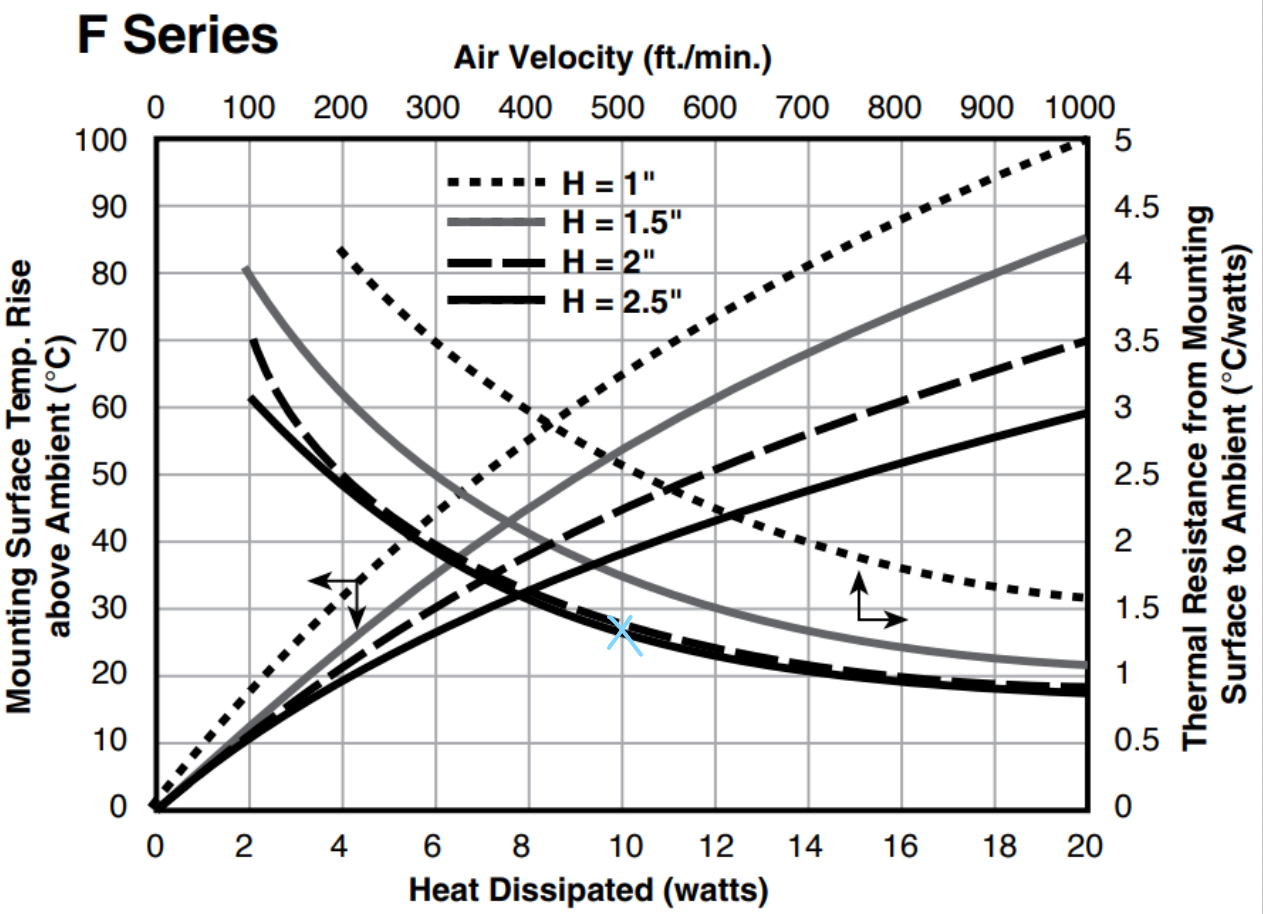
\includegraphics[width=0.3\textwidth]{F_series_heatsink_forces.png}
          \end{center}

          Assume air velocity of 500 ft/min gives 1.4$^{\circ}C/W$, with a 20\% safety factor. 
          \begin{align*}
          R_{\Theta sa} &= 1.4^{\circ}C/W \times 1.2 \\
          &=1.68^{\circ}C/W
          \end{align*}

          With new $R_{\Theta sa}$:
          \begin{align*}
            T &= R_{\Theta jc} \times P_{d} + (R_{\Theta cs} \times P_{d} + (R_{\Theta sa} \times P_{d} + T_{a})) \\
            &= 3.33*13+(0.2*13+(1.68*13+50)) \\
            &= 117.73^{\circ}C
          \end{align*}

          As shown, with the above scenario of forced convection, the temperature is brought under control.

\end{enumerate}

\section*{Question 3:}
\begin{enumerate}[label=\alph*)]
          \item
          \item
          \item
          \item
          \item
\end{enumerate}
\end{preview}
\end{document}